\newpage
\section{Auswertung}
\subsection{Emissionsspektrum}
\label{sub:emi}
\noindent
Aus den Messdaten aus Tabelle (\ref{tab:emi})lässt sich das Emissionsspektrum einer Kupferröntgenröhre in (\ref{fig:emi}) graphisch darstellen.

\noindent
Zu erkennen sind die ermittelten Peaks, die die $\text{K}_\alpha$ und $\text{K}_\beta$ Linie darstellen, sowie der orange makierte Bremsberg.

\begin{figure}
    \centering
       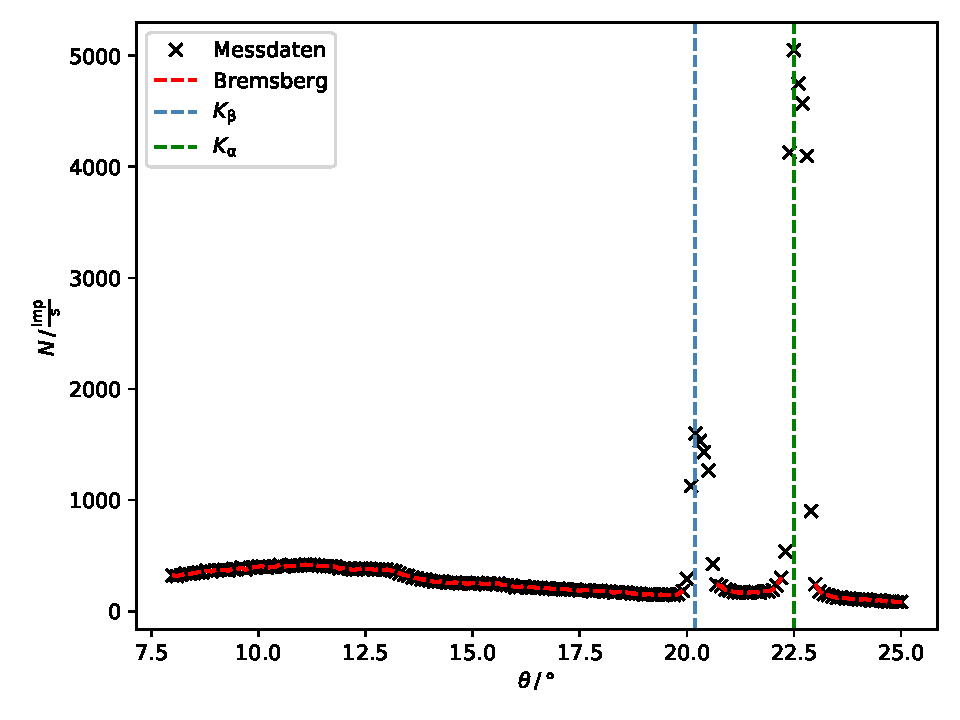
\includegraphics[height=9cm]{daten/emissionsspektrum.pdf}
       \caption{Emissionsspektrum einer Cu-Röntgenröhre.}
       \label{fig:emi}
\end{figure}

\noindent
Mittels Python lassen sich die Winkel zu den Peaks bestimen, woraus die Energie nach

\begin{equation}
    E = \frac{h \, c}{2 \, d_{LiF} \, \text{sin}\, (\theta)}
\end{equation}

\noindent
berechnet wird.

\begin{align*}
    \theta_\alpha&=20.2° & \theta_\beta&=22.5° \\
    \text{E}_\alpha&=8.0434 \, \mathrm{keV}   &\text{E}_\beta&=8.9142 \, \mathrm{keV} \\
\end{align*}

\newpage
\subsection{Bestimmung der Transmission}
Aus den gegebenen Zählraten $N$ aus Tabelle (\ref{tab:l_c}) lässt sich die Transmission $T$ mit

\begin{equation}
I = \frac{N}{1 - \tau \, N}
\label{eqn:tot}
\end{equation}

\noindent
mit der Totzeit $\tau = 90 \mu s$ und 

\begin{equation}
T = \frac{I_{Al}}{I_O}
\label{eqn:trans}
\end{equation}

\noindent
bestimmen.

\noindent
In Abbildung (\ref{fig:trans}) ist die Transmission mit dem Fehler $\Delta N = \sqrt{N}$ in Abhängigkeit von der Wellenlänge $\lambda$ aufgetragen.

\begin{figure}
    \centering
       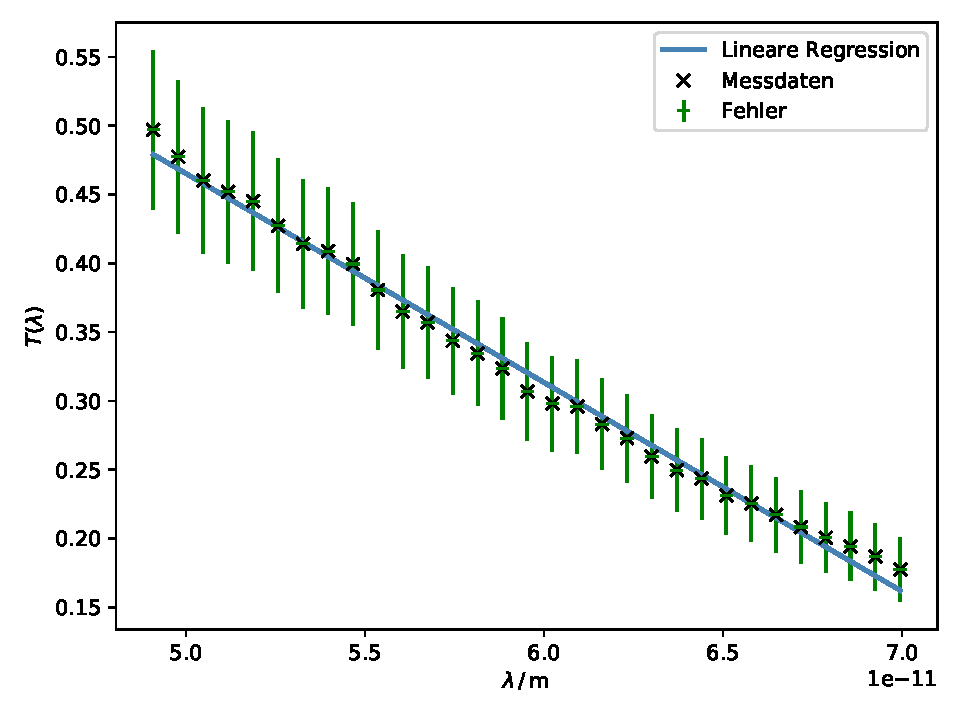
\includegraphics[height=9cm]{daten/transmission.pdf}
       \caption{Transmission.}
       \label{fig:trans}
\end{figure}

\noindent
Die Ausgleichsgerade der Form

\begin{equation*}
f(x) = m \cdot x + b
\end{equation*}

\noindent
lässt sich über polyfit bestimmen, sodass folgende Parameter ermittelt werden:

\begin{align*}
    m &= (-1.519 \pm 0.024)\cdot 10^{10} \\
    b &= 1.225 \pm 0.014 \\
\end{align*}

\subsection{Bestimmung der Compton-Wellenlänge}
Aus den gemessenen Impulsen 

\begin{align*}
    I_0 &= 2731 & &(\text{ohne Al-Absorber})\\
    I_1 &= 1180 & &(\text{mit Al-Absorber})\\
    I_2 &= 1024 & &(\text{mit Al-Absorber})\\  
\end{align*}

\noindent
werden die Transmissionen $T_1$ und $T_2$ mit Gleichung (\ref{eqn:trans}) bestimmt. So ergibt sich

\begin{align*}
    T_1 &= 0.432 \\
    T_2 &= 0.375.\\
\end{align*}

\noindent
Diesmal wird auf die Totzeitkorrektur nach Formel (\ref{eqn:tot}) verzichtet, da für kleine Zählraten $\tau \cdot N << 1$ gilt.

\noindent
Die zugehörigen Wellenlängen $\lambda_1$ und $\lambda_2$ lassen sich aus der Ausgleichsgeraden
mit 

\begin{equation*}
    \lambda = \frac{T - b}{m}
\end{equation*}

\noindent
zu

\begin{align*}
    \lambda_1 &= (5.22\pm 0.12)\cdot 10^{-11} \si{\meter}\\
    \lambda_2 &= (5.59\pm 0.13)\cdot 10^{-11} \si{\meter}\\
\end{align*}

\noindent
bestimmen.
Die Differenz $\Delta \lambda = \lambda_2 - \lambda_1 = \lambda_c$ ist dabei die Compton Wellenlänge

\begin{align*}
    \lambda_c =(3.76\pm 0.06)\cdot 10^{-12} \si{\meter}.
\end{align*}

